\section{Dihedral Groups and Group Generators}
\label{section_1.2}

Let $\Z^+$ and define $D_{2n}$ to be the set of symetries of a regular $n$-gon,
where a symmetry is just a permutation of the vertices. That is, if  $S$ is the
set of vertices, then a symmetry on  $S$ is just a map taking $S \rightarrow S$.
We would like to characterize the symmetries of $D_{2n}$ (See figure
\ref{fig_1.1}).

\begin{figure}
  \centering
  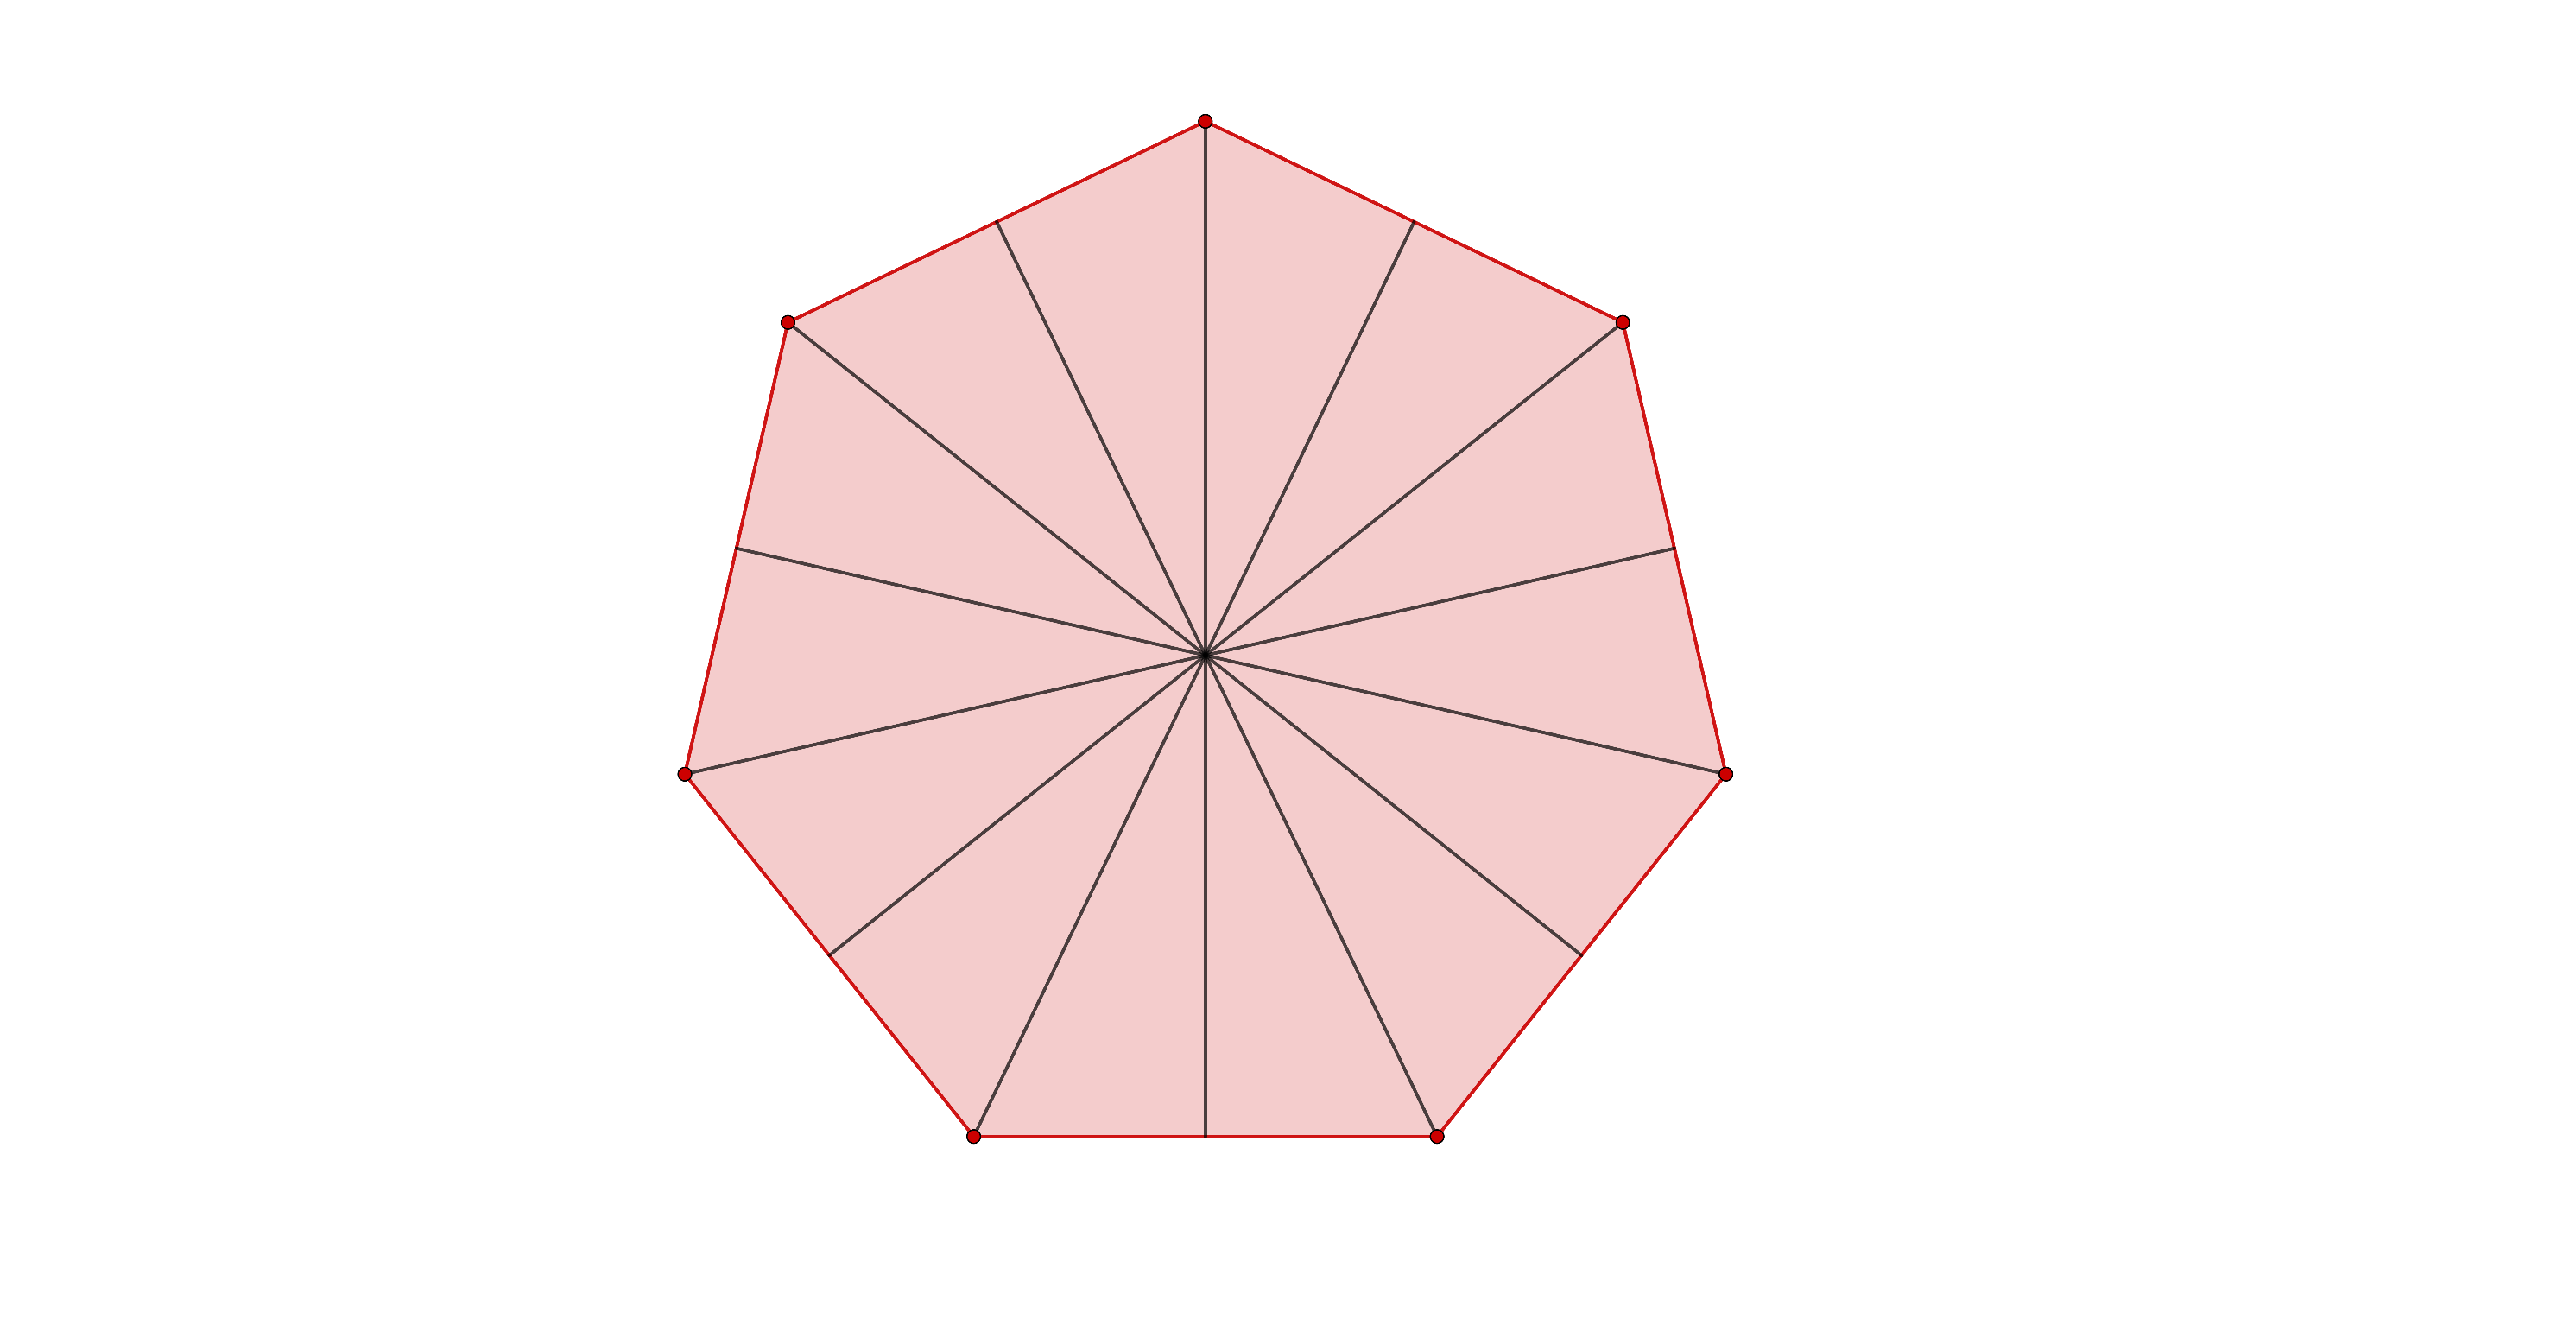
\includegraphics[scale=0.2]{parts/group_theory/figures/Chapter1/D_14_symm.eps}
  \caption{The group, $D_{14}$ of symmetries on a heptagon.}
  \label{figure_1.1}
\end{figure}

Since the set of vertices of the $n$-gon is arbitrary, but finite, we can label
$S$ how we see fit. Let us label $S = \faktor{\Z}{n\Z}$ and define the
symmetries
\begin{aligned}
  t:\faktor{\Z}{n\Z} & \xrightarrow{} \faktor{\Z}{n\Z}  \\
  i & \xrightarrow{} -i \\
\end{aligned}
and
\begin{aligned}
  r:\faktor{\Z}{n\Z} & \xrightarrow{} \faktor{\Z}{n\Z}  \\
  i & \xrightarrow{} i+1 \\
\end{aligned}
That is $t$ is a transposition  (or reflection) of the veritices, and $r$ is
a rotationif the vertices by an angle of  $\frac{2\pi}{n}$. Now, define
the ``identity'' symmetry $e:i \rightarrow i$. Then notice that
\begin{equation*}
  t^2:i \rightarrow -i \rightarrow -(-i)=i$, and $r^n:i \rightarrow i+1
  \rightarrow \dots \rightarrow i+n \equiv i
\end{equation*}
So $t^2=r^n=e$. (more over, if we treat $e$ as a rotation of the veritces by
an angle of  $2\pi$, then note that $r^n$ applies a rotation of the vertices by
an angle of  $\frac{2n\pi}{n}=2\pi$, which makes it the identity symmetry). It
is easy to see that $t$ and  $r$ are  $1-1$ and onto, so  $\inv{t}=t$ and
$\inv{r}=r^{n-1}$.

Now that we have characterized the symmetries $r$ and  $t$, what about  $r \circ
t$? Abbreviating  $r \circ t$ as  $rt$, we see that
\begin{equation*}
  rt:i \rightarrow -i \rightarrow -i+1=-(i+1)
\end{equation*}
Now, notice that
\begin{equation*}
  \inv{r}=r^{n-1}:i \rightarrow i+(n-1) \equiv i-1
\end{equation*}
Then
\begin{equation*}
  t\inv{r}:i \rightarrow i-1 \rightarrow -(i-1)=-i+1
\end{equation*}
Thus $rt=t\inv{r}$. This gives us the following lemma.

\begin{lemma}\label{lemma_1.2.1}
  For the symmetries $r$ and  $t$, and for  $i \in \faktor{\Z}{n\Z}$,
  $r^it=tr^{-i}$.
\end{lemma}
\begin{proof}
  By induction on $i$, we have for  $i=1$ that  $rt=t\inv{r}$. Now suppose for
  $i$ that  $r^it=tr^{-i}$. Then
  $r^{i+1}t=r(r^it)=(rt)r^{-i}=t\inv{r}r^{-i}=tr^{-i-1}=tr^{-(i+1)}$.
\end{proof}

We can now characterize the set $D_{2n}$.

\begin{definition}
  Let $S$ be a set of $n$ elements. We define the dihedral group
  $D_{2n}$ to be the set of all permutations on $S$ having the form $r^it^j$, where
  $i \in \faktor{\Z}{n\Z}$, $j \in \faktor{\Z}{2\Z}$, and where $r$ is
  a rotation about an angle of $\frac{2\pi}{n}$ and $t$ is a
  transposition. We write $D_{2n}=\langle r,t : r^n=t^2=e, \text{ and }, rt=t\inv{r}
  \rangle$.
\end{definition}

\begin{theorem}\label{theorem_1.2.2}
  $D_{2n}$ forms a group under function composition $\circ$, and the elements
  of $D_{2n}$ are of the forn $r^it^j$ with  $i \in \faktor{\Z}{n\Z}$ and $j
  \in \faktor{\Z}{2\Z}$.
\end{theorem}
\begin{proof}
  Since $r, t \in D_{2n}$, we have that $rt \in D_{2n}$ since $rt$ is also a
  permutation. Now by the above relations, we have that any element in
  $D_{2n}$ has the form $r^it^j$ where  $i \in \faktor{\Z}{n\Z}$ and $j \in
  \faktor{\Z}{2\Z}$. Now let $r^it^j, r^lt^k \in D_{2n}$ with $i,l \in
  \faktor{\Z}{n\Z}$ and $j,k \in \faktor{\Z}{2\Z}$. Then
  \begin{align*}
    (r^it^j)(r^lt^k)  &=  r^i(t^jt^k)r^{-l} \\
                      &=  r^it^{j+k}r^{-l}  \\
                      &=  (r^ir^l)t^{j+k} \\
                      &=  r^{i+l}t^{j+k}  \\
  \end{align*}
  Now, by the closure of both $\faktor{\Z}{n\Z}$, and
  $\faktor{\Z}{2\Z}$, we get that $r^{i+l}t^{j+k} \in D_{2n}$ which
  establishes closure of $D_{2n}$ under $\circ$. We also see that since
  $D_{2n}$ is a set of permutations, it inherits the associativity of $\circ$.

  Now consider the identity symmetry $e:i \rightarrow i$. We have $e=r^nt^2$,
  so for any  $r^it^j$,
  \begin{align*}
    (r^it^j)(r^nt^2)  &=  r^{i+n}t^{j+2}  \\
                      &=  r^ir^nt^jt^2  \\
                      &=  r^iet^je  \\
                      &=  r^it^j
  \end{align*}
  Likewise
  $(r^nt^2)(r^it^j)=(r^it^j)$. We also get that since $\inv{t}=t$ and
  $\inv{r}=r^{n-1}$ then if $s \in D_{2n}$, then $(r^it^j)s=e$ implies, by
  cancellation laws, that $s=t^jr^{-i}$, which serves as an inverse to
  $r^it^j$. Therefore  $D_{2n}$ is a group.
\end{proof}
\begin{corollary}
  $|D_{2n}|=2n$.
\end{corollary}
\begin{proof}
  We have that each element of $D_{2n}$ is of the form $r^it^j$ where $i \in
  \faktor{\Z}{n\Z}$ and $j=0$ or $j=1$. Thus there are two possible choices
  for $j$ and  $n$ possible choices for $i$, therefore there are  $2n$
  possible choices for  $r^it^j$, since this element is arbitrary, we have
  that this enumerates all the elements of  $D_{2n}$.
\end{proof}
\begin{corollary}
  $D_{2n}=\{e, t, r, r^2, \dots r^{n-1}, rt, r^2t, \dots, r^{n-1}t\}$.
\end{corollary}
\begin{proof}
  Compute each element  $r^it^j$, iterating over $i$ and  $j$.
\end{proof}

\begin{figure}
  \centering
  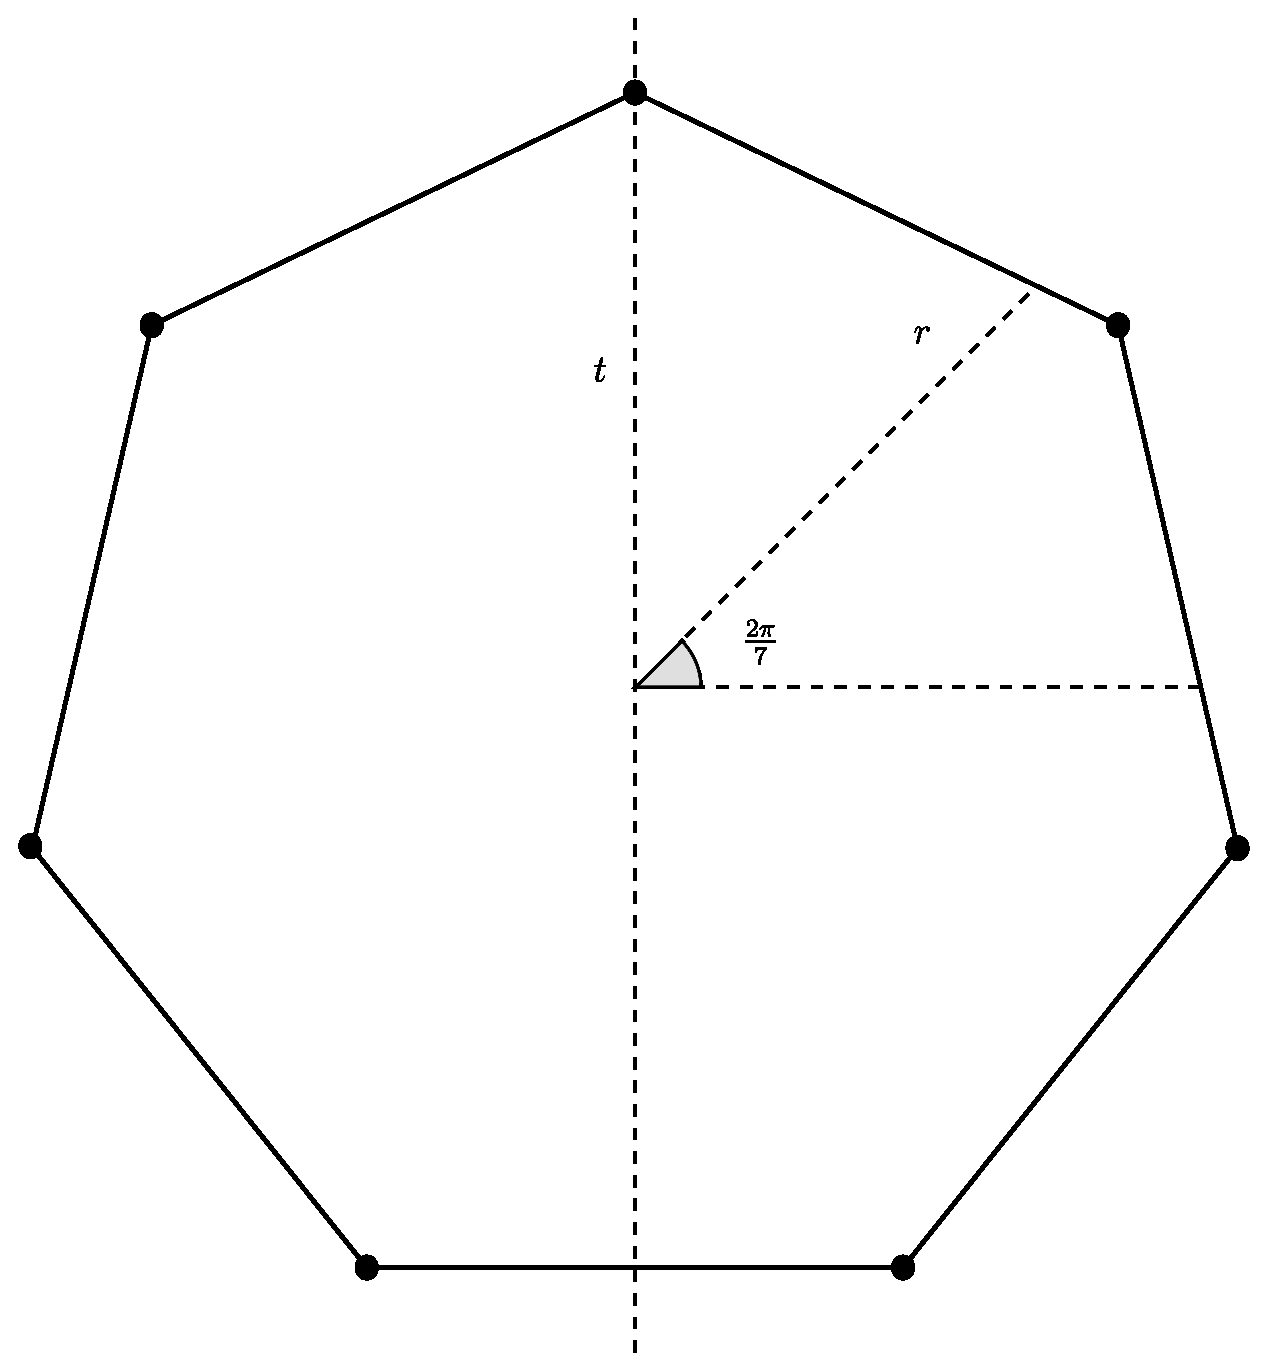
\includegraphics[scale=0.2]{parts/group_theory/figures/Chapter1/D_14.eps}
  \caption{The transposition $t \in D_{14}$ of vertices of a heptagon and the
  rotation $r \in D_{14}$ about an angle of $\frac{2\pi}{7}$ of the vertices.}
  \label{figure_1.1}
\end{figure}

Thus we have entirely described the set of symmetries of a regular $n$-gon in
group theoretic terms; and have found that they follow a certain  (special case,
of a more general) group structure. In fact, we have found elementd $r,t$ that
``generate'' the symmetries, and found relations which we can use to describe
the group. This leads us to the following definition.

\begin{definition}
  Let $G$ be a grou p. We say that a subset, $S \subseteq G$
  \textbf{generates} the group $G$ if for every  $g \in G$,  $g$ is the finite
  product of elements of  $S$. We write  $G=\langle S \rangle$ and call $S$ the
  \textbf{generator} of $G$. If the elements of  $S$ satisfy a set of
  relations  $R_1, \dots R_n$, then we say $G$ is  \textbf{represented} by $S$
  by $R_1, \dots R_n$ and write $G=\langle S : R_1, \dots, R_n \rangle$, and call
  this form the \textbf{representation} of $G$.
\end{definition}

\begin{example}
  \begin{enumerate}
    \item[(1)] $\Z= \langle 1 \rangle$.

    \item[(2)] $\faktor{\Z}{n\Z}=\langle 1 \rangle$.

    \item[(3)] $D_{2n}= \langle r,t : r^n=t^2=e \text{ and }
      rt=t\inv{r} \rangle$.

    \item[(4)] Define $X_{2n}=\langle x,y : x^n=y^2=e, xy=yx^2 \rangle$. Since
      $y^2=e$, we have  $x=xy^2=(xy)y=y(x^2y)=y^2x^4=x^4$; thus $x^4=x$,
      hence  $x^3=e$. Therefore  for any $n$, $|X_{2n}|=6$, by the
      same argument we made for $D_{2n}$.

    \item[(5)] Let $Y=\langle u,v : u^4=v^3=e, uv=v^2u^2 \rangle$. We have
      $u=uv^3=v^6u^2=(v^3)^2u^2=e^2u^2=u^2$, hence $u^2=u$, hence  $u=e$;
      thus we also get that  $v^2=v$, hence  $v=e$. Therefore
      $Y=\langle e \rangle$, the trivial group.
  \end{enumerate}
\end{example}

The previous two examples show that not every relation may be listed in the
representation of a given group. It turns out in the case of $D_{2n}$, that all
the relations are listed, but as in the above example with $X_{2n}$ and $Y$, we
had the relations $x^4=x$ and  $u^2=u, v^=v$. Thus one may be careful when
dealing with group representations and take care that no relations are left
unattended. One consequence might be an erroneous arguing of group order; one
can be led to believe that $|X_{2n}|=2n$, where in reality $|X_{2n}|=6$
and that $|Y|=6$, where in reality, $|Y|=1$.
